% Pursuing Stacks (cotes 134-2 to 134-8): archive cote 134-3, site page 10 (PDF page 11), typescript page 10.
% typescript. Draft compared: ps2.tex:415-483.
% AI-transcribed by Claude Opus 5.5 (claude-opus-5-5, adaptive thinking, effort high), Message Batches API, batch ps1 (msgbatch_01Rv5hCaNTtUt4JHx1yqoHPL), 2026-11-12; image review recorded in records/CHECK_DECISIONS_134_3_4.tsv.
\scanpage{134-3/10}
\mspage{\hand{10}}

28.2.

\over{\unsure{18}}{18}. I still have to correct a number of ``étourderies'' of (L). The
most persistent one, ever since page 8 of that letter, is about fiber
products in the coherator $\underline{C}_\infty$ , or, equivalently, amalgamated sums in
the dual category $\underline{B}_\infty$ . The ``correction'' I added in the last PS \inserted{(section 13)} \deleted{\unsure{p.11'}} is
still incorrect, namely it is not true \xout{thatxix} even in the subcategory
$\underline{B}_o$ of $\underline{B}$ that arbitrary binary amalgamated sums exist. I was mislead
by the interpretation of elements of $\underline{B}_o$ in terms of \inserted[typed]{(contractible)} spaces\hand{,} obtained
inductively by gluing together discs $D_n$ ($n \in \underline{N}$) via subdiscs, correspon-%
ding to the cellular subidivisions of the discs $D_n$ considered on p.7.
I was implcitly thinking of amalgamated sums of the type
\[ K \amalg_L M \quad , \]
where $L$ \hand{$\to$} $K$ and $M$ \hand{$\to$}\xout{x}$K$ are \uline{monomorphisms}, corresponding to the geometric
vision of embeddings - in which case the usual amalgamated sum in the
category of topological spaces is indeed contractible, wh\over{\unsure{at}}{ich} was enough
to make me happy. But I overlooked the existence of morphisms in $\underline{B}_o$
which are visibly no monomorphisms, such as $K \amalg_L K$ \hand{$\to$} $K$ the codiaganal
map, when $L$ \hand{$\to$}$K$ is a\xout{n} \inserted[typed]{strict} inclusion of discs\xout{x} . In any case, I will have
to come back upon the description of the categories $\underline{B}_o$ and it's dual $\underline{C}_o$ ,
and upon the definition of coherators, after the heuristic introduction
(L). It will be time then \inserted{too} to correct the mistaken description of $\underline{C}_{n+1}$
in terms of $\underline{C}_n$ , which I propose \inserted{there} \deleted{on p.11'}, yielding probably much too
big a subcategory of $\underline{C}$\xout{xxxx}\hand{$_\infty$} - the correct definition should make explicit
use of the \inserted[typed]{total} set A of \xout{xxxxxx} ``new'' arrows, by which $\underline{C}_\infty$ is described in
terms of universal algebra via $\underline{C}_o$ . Another étourderie the day before\hand{,}
\inserted{(section 7)} \deleted{p.7'}, is the statement that in a standart amalgamated sum, an\over{d}{y} inter-%
section of two \inserted[typed]{maximal} subcells is a subcell - which is seen to be false in
\margin{\diagram{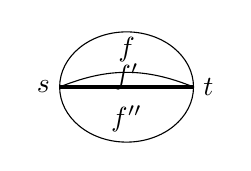
\begin{tikzpicture}[x=1cm,y=1cm,baseline=(current bounding box.center)] \draw (0,0) ellipse (0.85 and 0.70); \draw (-0.85,0) to[bend left=22] (0.85,0); \draw[line width=1.1pt] (-0.85,0)--(0.85,0); \node at (0,0.48) {$f$}; \node at (0,0.13) {$f'$}; \node at (0,-0.40) {$f''$}; \node[left] at (-0.85,0) {$s$}; \node[right] at (0.85,0) {$t$}; \end{tikzpicture}} $f\cap f''=\{s,t\}$} \deleted{the}\inserted{a} standard example\hand{.} \hand{\unsure{$\ell$}} \over{o}{O}f lesser import is the misstatement \inserted{(in section 2)} \deleted{on p.2'},
stating that the associativity relation for the operation \hand{$*_\ell$} should be
\xout{wherex\allowbreak{}fx\allowbreak{}f"x\allowbreak{}isx\allowbreak{}ax\allowbreak{}two-pointx\allowbreak{}spacex\allowbreak{}$\underline{S}_o$x\allowbreak{}x\allowbreak{}x\allowbreak{}} replaced by a homotopy arrow
$(\hand{\lambda}*\hand{\mu})*\hand{\nu} \to \hand{\lambda}*(\hand{\mu}*\hand{\nu})$. This is OK for \hand{$\ell$}=1 (primary composition), but
already for \hand{$\ell$}=2 does not make sense as stated, because the sources and
the targets of the two compositions to be compared are not equal, but
only homotopic. Here the statement should be replaced by one making
sense, with a homotopy ``making commutative'' a certain square, and accor\hand{\unsure{-}}%
dingly for cubes etc for higher order co\xout{mp}mpositions \hand{$\lambda *_\ell \mu$}, to give rea-%
sonable meaning to associativity. Anyhow, such painstaking explicita-%
tions of particular coherence properties (rather, coherence homotopies)
is kind of ruled out by the sweeping axiomatic description of the
kind of structure species we want for a ``stack'', at least\hand{,} I guess\hand{,} in
